\documentclass[10pt]{beamer}

\usetheme{Boadilla}

\usepackage{pgf}
\usepackage[english]{babel}
\usepackage[utf8]{inputenc}

\usepackage{bm}
\usepackage{tikz}

\usepackage{times}
\usepackage[T1]{fontenc}

\definecolor{basecolor}{RGB}{79, 17, 32}

\title[\pgfuseimage{department-logo}] %
{Un modelo de Markov para la segmentación automática de señales de audio}

\author[Rafael de Jesús Robledo Juárez] %
{Rafael de Jesús Robledo Juárez \\
\small{\texttt{rrobledo@cimat.mx}} \\ ~\\
\small{Asesor: Dr. Salvador Ruíz Correa}}


\institute[CIMAT]
{
  Departamento de Ciencias de la Computación\\
  Centro de Investigación en Matemáticas, Guanajuato \\
  ~ \\
  \pgfuseimage{university-logo}
}

\date[Febrero 2013]
{Presentación de Avance de Tesis, 2013}
\subject{Latex Beamer Template}

\pgfdeclareimage[interpolate=true, height=2.5cm]{university-logo}{logos/logo-big}
\pgfdeclareimage[interpolate=true, height=0.6cm]{department-logo}{logos/logo-trans}
%\logo{\pgfuseimage{department-logo}}

\usecolortheme[named=basecolor]{structure} 
\setbeamertemplate{navigation symbols}{} 

\begin{document}

\newcommand*\actwidth{8cm}
\newcommand*\actheight{1.6em}

\tikzset{entry/.style 2 args={
    xshift=(0.5334em+0.8pt)/2,
    draw,
    font=\sffamily,
    rectangle,
    rounded corners,
    fill = basecolor!70,    
    anchor=north west,
    line width=0.1pt,
    inner sep=0.3333em,
    text width={\actwidth/#2-1.2em-1.6pt},
    minimum height=#1*\actheight,
    align=center
}}

\setbeamertemplate{itemize items}[default]
\setbeamertemplate{enumerate items}[default]
\setbeamerfont{section number projected}{series=\bfseries,size={\fontsize{8}{12}}}
\setbeamertemplate{sections/subsections in toc}[square]

\begin{frame}
  \titlepage
\end{frame}

\section{Introducción}

\subsection{Objetivo}

\begin{frame}{Objetivo}
  \begin{itemize}
  	\item
       Utilizar un modelo del tipo HMM (\textit{Hidden Markov Model} por sus siglas en Inglés) 
       por medio del cual sea posible particionar una secuencia de audio en regiones homogéneas.
       Cada región debe corresponder con la identidad de un hablante. 
       
     \item
       A esta tarea se le conoce con el nombre de \textit{"speaker diarisation"}.

       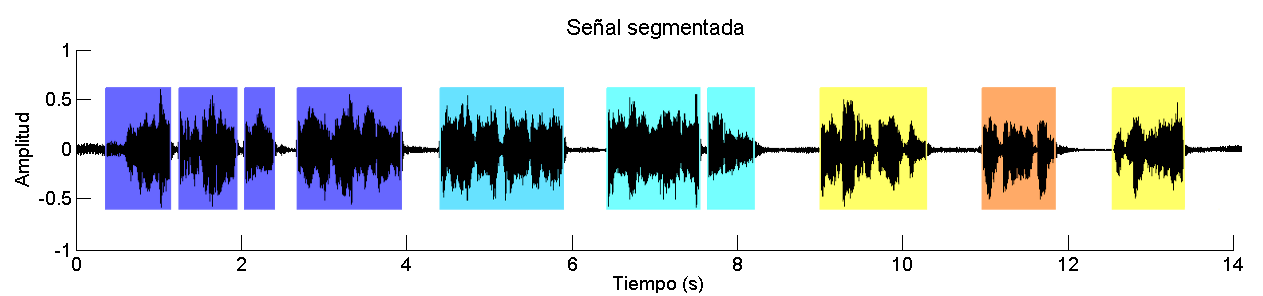
\includegraphics[width=0.9\textwidth]{gfx/f-segm}

  	\item	
  	  Los segmentos obtenidos se etiquetarán de acuerdo a cada persona diferente que se identifique.
  \end{itemize}
\end{frame}

\subsection{Motivación}

\begin{frame}{Motivación}
  \begin{itemize}
    \itemsep 2.5em  
    \item La identificación de las personas que participan en una grabación de audio, 
    es una etapa importante en aplicaciones tales como transcripción automática
    y reconocimiento de voz.
    
    \item Un paso importante para la automatización de este proceso, consiste en poder segmentar
    la señal de audio sin necesidad de conocimiento a priori sobre el número o género de las personas
    involucradas en la grabación.
    
  \end{itemize}
\end{frame}

\section{Metodología}

\subsection{Procesamiento de señal}

\begin{frame}{Metodología}{Procesamiento de señal}
\small {
\vspace{0mm} 
\begin{columns}   
  \begin{column}{0.6\textwidth} 
    \hfill  
    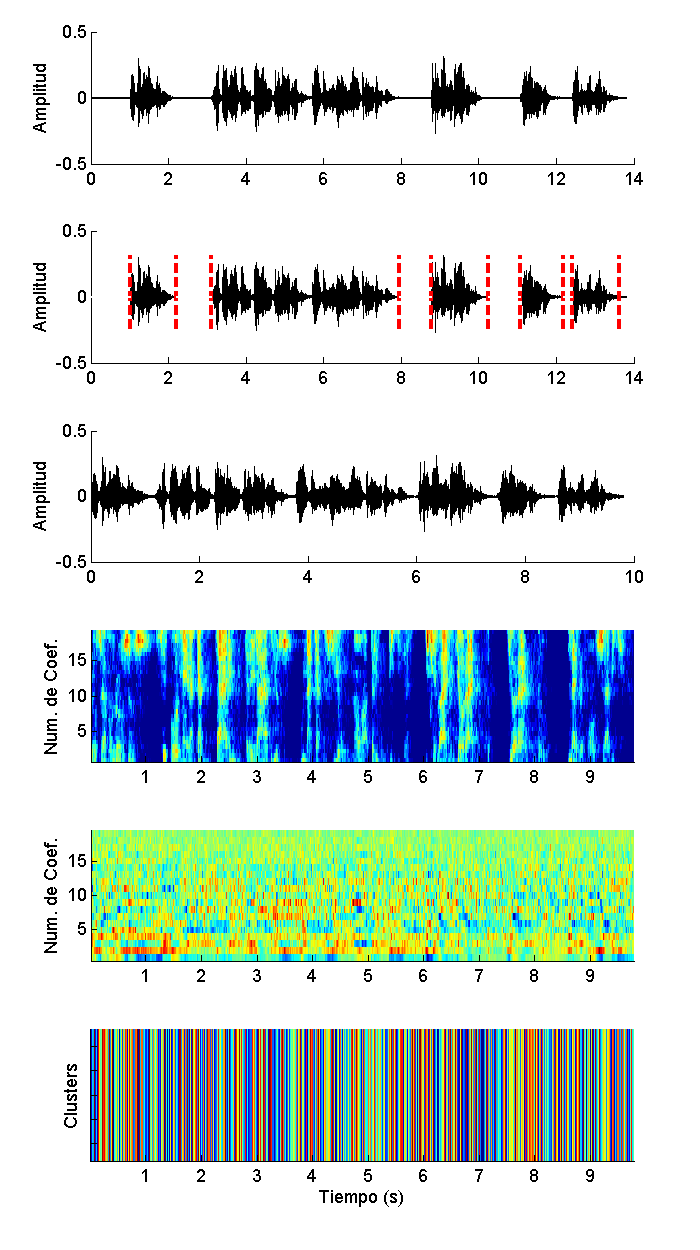
\includegraphics[width=0.64\textwidth]{gfx/filename5}    
  \end{column}
  \begin{column}{0.4\textwidth}
    \vspace{-8mm} 
    \begin{itemize}
      \setlength{\itemindent}{-2em}      
      \itemsep 2.7em    
      \item Señal original
      \item Identificación de silencios
      \item Señal de audio recortada
      \item FFT + Banco de filtros + log
      \item MFCC
      \item k-means
    \end{itemize}
  \end{column}   
\end{columns}   
}
\end{frame}

\subsection{Modelo}
\begin{frame}{Metodología}{Modelo}
  \begin{center}
    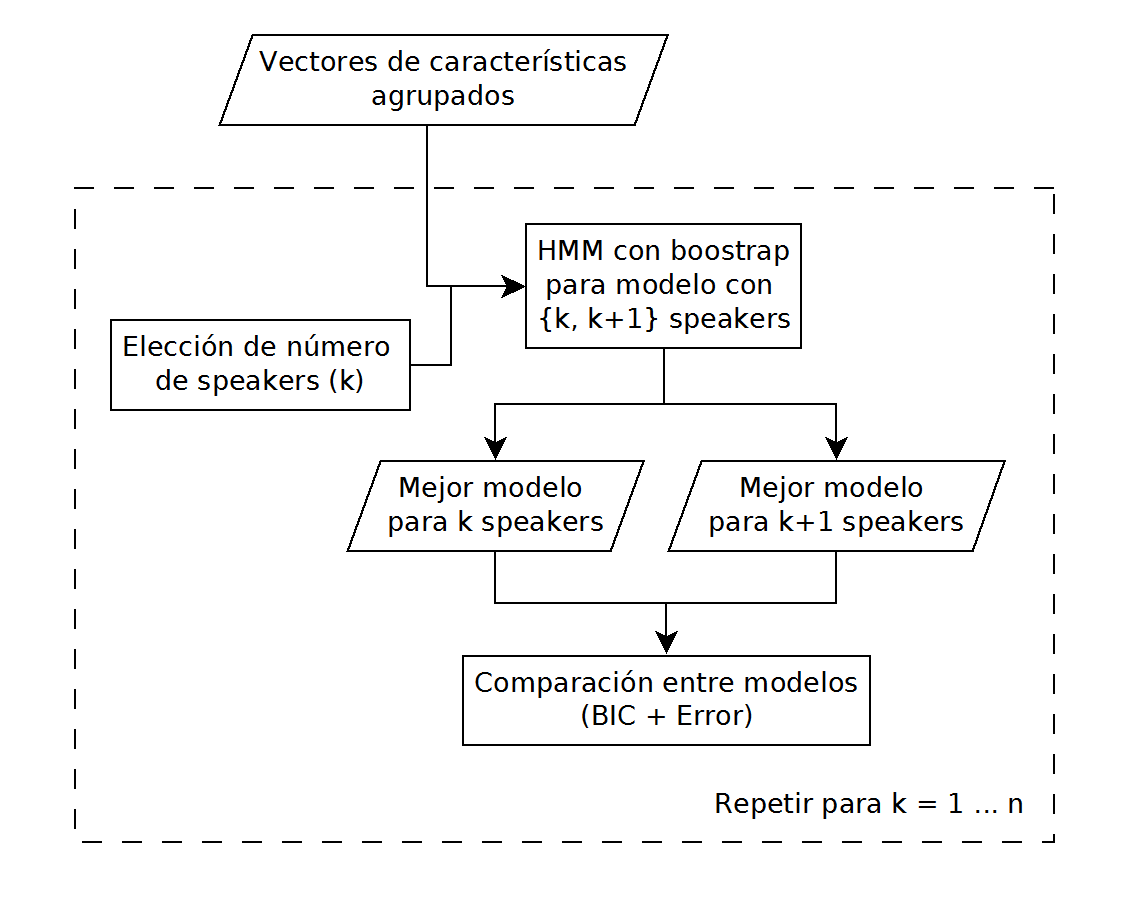
\includegraphics[width=0.7\textwidth]{gfx/dia-hmm}
  \end{center}
\end{frame}

\section{Avances}
\begin{frame}{Avances}
  \begin{itemize}
    \itemsep 3em
    \item Implementación completa del sistema.
    \item Resultados con datos sintéticos.
    \item Pruebas con datos reales.
  \end{itemize}
\end{frame}

\section{Resultados}
\subsection{Pruebas con datos sintéticos}
\begin{frame}{Pruebas con datos sintéticos}
  \begin{center}
    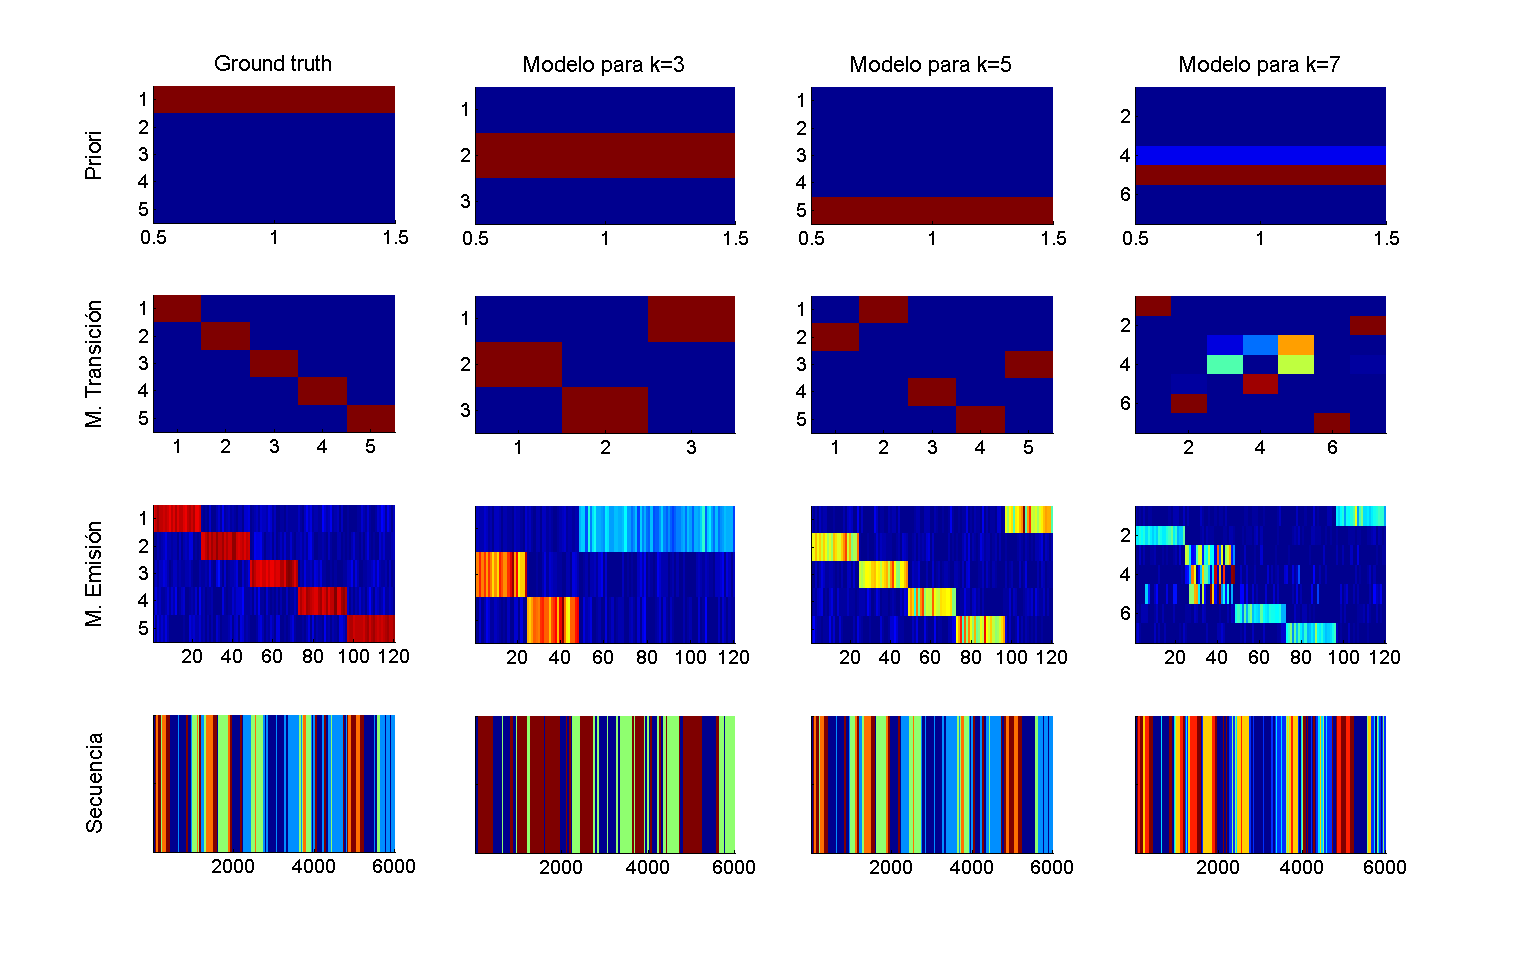
\includegraphics[height=0.65\textwidth]{gfx/pruebasg}
  \end{center}
\end{frame}

\begin{frame}{Pruebas con datos sintéticos}
  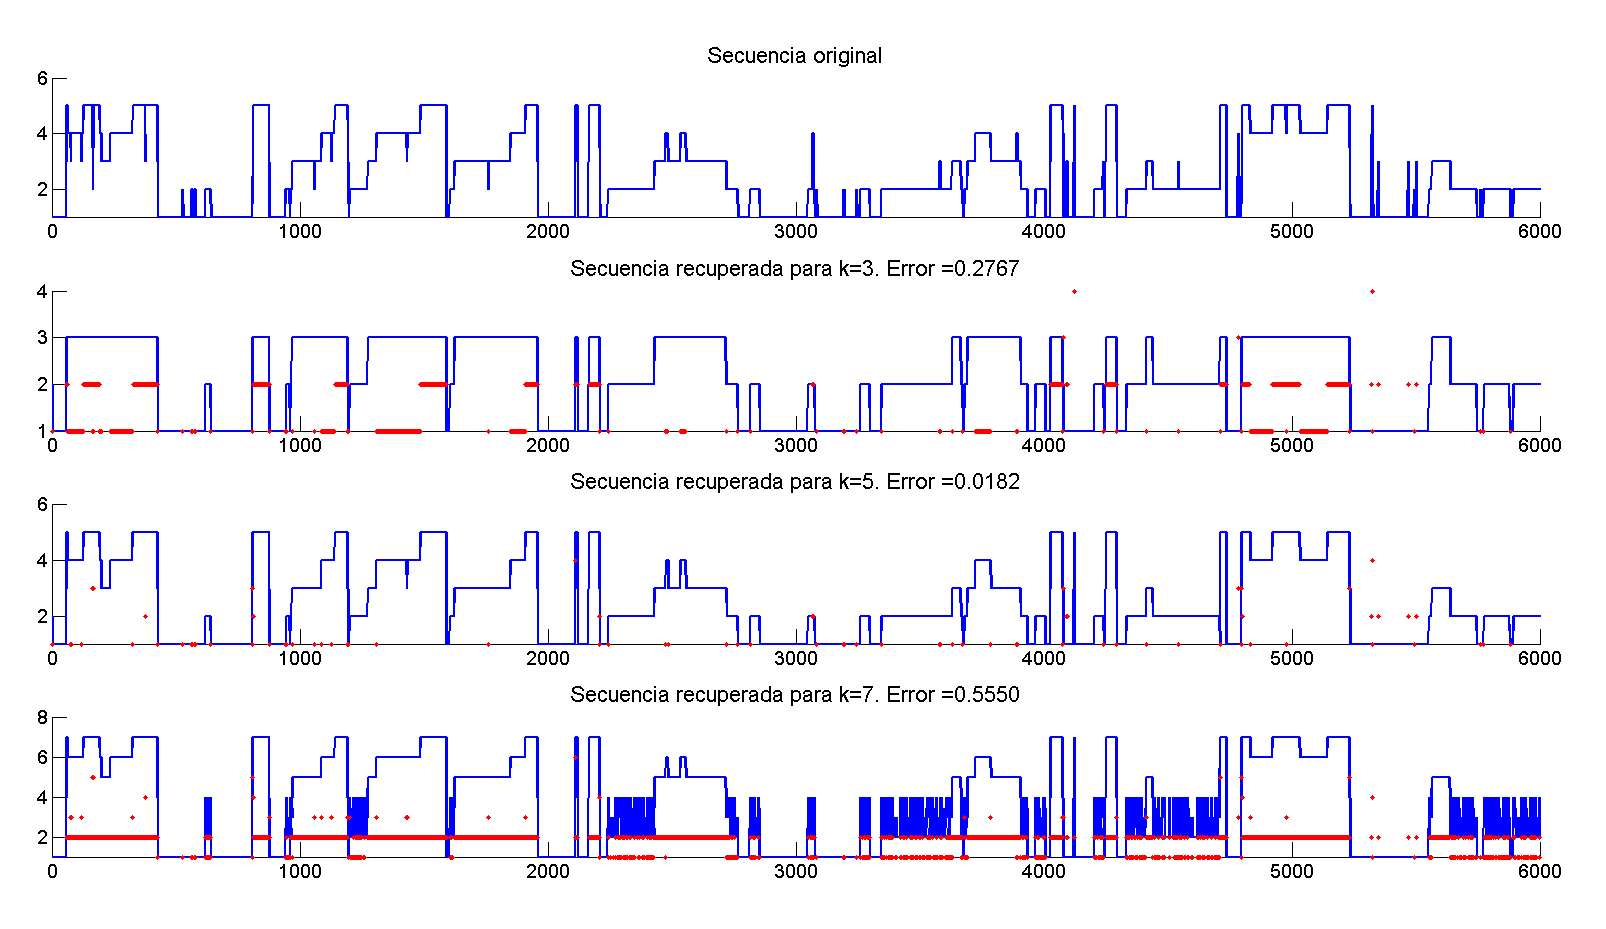
\includegraphics[height=0.6\textwidth]{gfx/pruebasg_}
\end{frame}

\section{Calendario}
\begin{frame}{Calendario}

\begin{center}
\begin{tikzpicture}[y=-\actheight,x=\actwidth]
    % First print a list of times.
    \foreach \nmonth/\Month in {2/Febrero, 3/Marzo, 4/Abril, 5/Mayo, 6/Junio, 7/Julio}
        \node[anchor=north east] at (1, \nmonth) {\Month};

    \node[anchor=north] at (1.5, 0) {\large{Actividades}};

    \node[entry={2.5}{2}] at (1.0, 2.4) {Pruebas con datos reales};
    \node[entry={2.5}{2}] at (1.5, 3.5) {Comparación y análisis de resultados};
    \node[entry={2.0}{2}] at (1.0, 5.0) {Escritura y revisión};
  \end{tikzpicture}

\end{center}
\end{frame}

\section{Apéndice}
\subsection{Material de consulta}

\begin{frame}{Material de consulta}
  
  \footnotesize {
  \begin{thebibliography}{10}
    
  \beamertemplatebookbibitems

  \bibitem{Bishop} 
  {L.R. Rabiner, B.H. Juang}
    \newblock \em{Fundamentals of speech recognition}
    \newblock Pearson Education India, 2008.
  
  \bibitem{Bishop}
    {C. M. Bishop.}
    \newblock \em{Pattern Recognition and Machine Learning}.
    \newblock Springer, 2006.
     
  \beamertemplatearticlebibitems
    
  \bibitem{Lawrence}
    {L.R. Rabiner}
    \newblock \em{A tutorial on hidden Markov models and selected 
      applications in speech recognition}
    \newblock Proceedings of the IEEE, 1989.

  \bibitem{Ryden}
    {T. Rydén.}
    \newblock \em{Versus Markov chain Monte Carlo for Estimation of Hidden 
    Markov Models: A Computational Perspective}
    \newblock {Bayesian Analysis (2008) 3}, Number 4, p. 659-688
    
  \bibitem{Emily}
    {E.B. Fox, E.B. Sudderth, M.I. Jordan, A.S. Willsky.}
    \newblock \em{A sticky HDP-HMM with application to Speaker diarization}.
    \newblock {Annals of Applied Statistics}, 2011.
     
  \end{thebibliography}
  }
\end{frame}

\end{document}